\section{Đề ôn thi giữa kỳ 2 toán 10}

\subsection{Phần trắc nghiệm}
Câu trắc nghiệm nhiều phương án lựa chọn. Học sinh trả lời từ
câu 1 đến câu 12. Mỗi câu hỏi học sinh \textit{chỉ chọn một} phương án.

\Opensolutionfile{ans}[Ans/Dapan]

\hienthiloigiaiex
%%%=============EX_1=============%%%
\begin{ex}%[0D3N1-5]%[Dự án đề kiểm tra Toán khối 10 GHKII NH23-24-Dot 2- Nguyễn Hữu Đức]%[Deso6 - KNTT]
	\immini{
		Cho hàm số $y=f(x)=x^2$ có đồ thị như hình bên. Khẳng định nào sau đây là \textbf{đúng}?
		\choice
		{Hàm số đồng biến trên $ \mathbb{R} $}
		{\True Hàm số đồng biến trên $(0;\infty)$}
		{Hàm số nghịch biến trên $ \mathbb{R} $}
		{Hàm số đồng biến trên $(-\infty;0)$}
	}{
		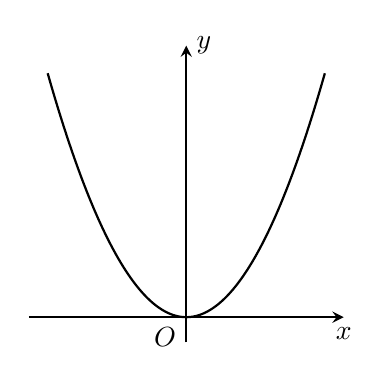
\begin{tikzpicture}[>=stealth, scale=.8,samples=200,xscale=1,yscale=.8,line width=.8pt]
			\draw[->,thick] (-2.5,0)--(2.5,0) node[below] {$x$};
			\draw[->,thick] (0,-0.5)--(0,5.39)node[right] {$y$};
			\draw (0,0) node [below left]{$O$};
			\def\f(#1){(#1)^2}
			\draw[domain=-2.2:2.2,smooth,variable=\x,thick]plot (\x,{\f(\x)});
		\end{tikzpicture}
	}
	\loigiai{
		Dựa vào đồ thị hàm số $ y=x^2 $, ta thấy hàm số đồng biến trên $(0;\infty)$.}
\end{ex}
%%%=============EX_2=============%%%
\begin{ex}%[0D3H1-2]%[Dự án đề kiểm tra Toán khối 10 GHKII NH23-24-Dot 2- Nguyễn Hữu Đức]%[Deso6 - KNTT]
	\immini{
		Cho hàm số $y=f(x)$ có đồ thị như hình bên.
		Tập xác định của hàm số là
		\choice
		{$D=[-1;4]$}
		{\True $D=[-3;3]$}
		{$D=[-3;4]$}
		{$D=(-\infty ; +\infty)$}}
	{
		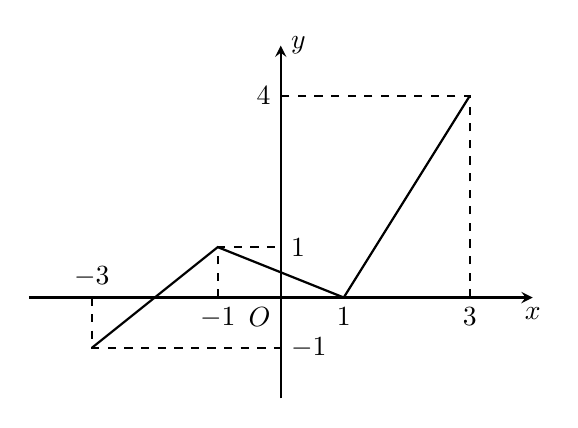
\begin{tikzpicture}[>=stealth, scale=.8,samples=200,xscale=1,yscale=.8,line width=.8pt]
			\draw[->,thick] (-4,0)--(4,0) node[below] {$x$};
			\draw[->,thick] (0,-2)--(0,5)node[right] {$y$};
			\draw (0,0) node [below left]{$O$};
			\draw[dashed](-3,0)node[above]{$-3$}|-(0,-1)node[right]{$-1$} (-1,0)node[below]{$-1$}|-(0,1)node[right]{$1$} (3,0)node[below]{$3$}|-(0,4)node[left]{$4$} (1,0)node[below]{$1$};
			\draw(-3,-1)--(-1,1)--(1,0)--(3,4);
		\end{tikzpicture}
	}
	\loigiai{
		Dựa vào đồ thị tập xác định hàm số là $D=[-3;3]$.
	}
\end{ex}
%%%=============EX_3=============%%%
\begin{ex}%[0D3H1-5]%[Dự án đề kiểm tra Toán khối 10 GHKII NH23-24-Dot 2- Nguyễn Hữu Đức]%[Deso6 - KNTT]
	Chọn từ thích hợp điền vào chỗ $ (\cdots) $. Đồ thị hàm số $ y=-5x^2+4x $ là một Parabol có bề lõm $\cdots$
	\choice
	{\True quay lên}
	{quay xuống}
	{quay sang trái}
	{quay sang phải}
	\loigiai{
		Ta có: $y=-5x^2+4 x$ có $a=-5<0$ nên bề lõm quay lên.
	}
\end{ex}
%%%=============EX_4=============%%%
\begin{ex}%[0D3H1-1]%[Dự án đề kiểm tra Toán khối 10 GHKII NH23-24-Dot 2- Nguyễn Hữu Đức]%[Deso6 - KNTT]
	\immini{
		Cho hàm số $y=a x^2+b x+c$ có đồ thị như hình bên. Khi đó $ 2a+b+2c $ có giá trị là
		\choice
		{$-9$}
		{$9$}
		{\True $-6$}
		{$6$}
	}{
		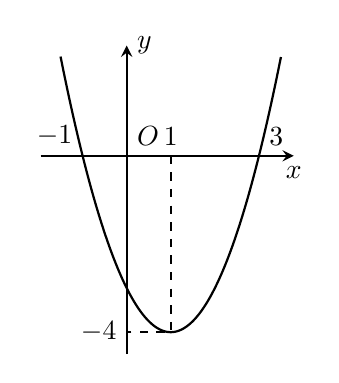
\begin{tikzpicture}[>=stealth, scale=.8,samples=200,xscale=0.7,yscale=.7,line width=.8pt]
			\draw[->,thick] (-1.95,0)--(3.79,0) node[below] {$x$};
			\draw[->,thick] (0,-4.5)--(0,2.5)node[right] {$y$};
			\draw (0,0) node [above right]{$O$};
			\draw (-1,0) node [above left]{$-1$};
			\draw (3,0) node [above right]{$3$};
			\draw[dashed]
			(1,0) node[above]{$1$}--(1,-4)--(0,-4) node[left]{$-4$};
			\def\f(#1){(#1)^2-2*(#1)-3}
			\draw[domain=-1.5:3.5,smooth,variable=\x,thick]plot (\x,{\f(\x)});
		\end{tikzpicture}
	}
	\loigiai{
		Dựa vào đồ thị ta thấy $a>0$, đồ thị hàm số cắt trục hoành tại 2 điểm, nên phương trình $a x^2+b x+c=0$ có 2 nghiệm $ x_1=-1,x_2=3 $ và đồ thị đi qua điểm $ I(1;-4) $ do đó\\
		\[\heva{&y(-1)=0\\&y(3)=0\\&y(1)=-4}\Leftrightarrow \heva{&a-b+c=0=0\\&9a+3b+c=0=0\\&a+b+c=-4}\Leftrightarrow \heva{&a=1\\&b=-2\\&c=-3.}\]
		Vậy $ y=x^2-2x-3 $. Khi đó $ 2a+b+2c=-6 $. 
	}
\end{ex}
%%%=============EX_5=============%%%
\begin{ex}%[0D7H1-2]%[Dự án đề kiểm tra Toán khối 10 GHKII NH23-24-Dot 2- Nguyễn Hữu Đức]%[Deso6 - KNTT]
	Dấu tam thức bậc hai $ f(x)=-x^2+5x-6 $ được xác định như sau
	\choice
	{$f(x)<0$ với $ 2<x<3 $, $ f(x)>0 $ với $ x<2 $ hoặc $ x>3 $}
	{$f(x)<0$ với $ -3<x<-2 $, $ f(x)>0 $ với $ x<-3 $ hoặc $ x>-2 $}
	{\True $f(x)>0$ với $ 2<x<3 $, $ f(x)<0 $ với $ x<2 $ hoặc $ x>3 $}
	{$f(x)>0$ với $ -3<x<-2 $, $ f(x)<0 $ với $ x<-3 $ hoặc $ x>-2 $}
	\loigiai{
		Xét $-x^2+5x-6=0 \Leftrightarrow \hoac{&x=2 \\& x=3.}$ \\
		Bảng xét dấu
		\begin{center}
			\begin{tikzpicture}
				\tkzTabInit[nocadre=false,lgt=2.5,espcl=2.5,deltacl=0.6,lw=.8]
				{$x$ /.6, $-x^2+5x-6$/0.6}{$-\infty$,$2$,$3$,$+\infty$}
				\tkzTabLine{,-,0,+,0,-,}
			\end{tikzpicture}
		\end{center}
		Ta có: $f(x)>0$ với $ 2<x<3 $, $ f(x)<0 $ với $ x<2 $ hoặc $ x>3 $}
\end{ex}
%%%=============EX_6=============%%%
\begin{ex}%[0D7H3-1]%[Dự án đề kiểm tra Toán khối 10 GHKII NH23-24-Dot 2- Nguyễn Hữu Đức]%[Deso6 - KNTT]
	Tập nghiệm phương trình $\sqrt{x^2-2 x}=\sqrt{2x-x^2}$ có nghiệm là
	\choice
	{$T=\{0\}$}
	{$T=\emptyset$}
	{\True $T=\{0;2\}$}
	{$T=\{2\}$}
	\loigiai{
		\begin{align*}
			\sqrt{x^2-2 x}=\sqrt{2x-x^2} \Leftrightarrow \heva{&2x-x^2 \geq 0\\& x^2-2x = 2x-x^2}\Leftrightarrow\heva{&0\le x \le2\\&\hoac{&x=0\,\text{(nhận)}\\&x=2\,\text{(nhận)}}}\Leftrightarrow x=2,\,x=0.
		\end{align*}
	}
\end{ex}
%%%=============EX_7=============%%%
\begin{ex}%[0H9H3-2]%[Dự án đề kiểm tra Toán khối 10 GHKII NH23-24-Dot 2- Nguyễn Hữu Đức]%[Deso6 - KNTT]
	Phương trình đường thẳng cắt hai trục tọa độ tại 2 điểm $A(-2 ; 0)$ và $B(0 ; 5)$ là
	\choice
	{$\dfrac{x}{2}-\dfrac{y}{5}=1$}
	{$\dfrac{x}{-2}-\dfrac{y}{5}=1$}
	{\True $5x+2y-10=0$}
	{\True $5x-2y+10=0$}
	\loigiai{
		Đường thẳng đã cho có một vectơ chỉ phương là $\overrightarrow{A B}=(2 ; 5)$.\\
		Vì vậy đường thẳng có một vectơ pháp tuyến là $\overrightarrow{n}=(-5 ; 2)$.\\
		Phương trình đường thẳng $ -5(x+2)+2(y-0)=0\Leftrightarrow -5x+2y-10=0 $ $\Leftrightarrow 5x-2y+10=0$.}
\end{ex}
%%%=============EX_8=============%%%
\begin{ex}%[0H9H3-2]%[Dự án đề kiểm tra Toán khối 10 GHKII NH23-24-Dot 2- Nguyễn Hữu Đức]%[Deso6 - KNTT]
	Phương trình tham số của đường thẳng $ d $ đi qua điểm $M(3;-4)$ và song song 
	đường thẳng $ d_1:\dfrac{x-7}{2}=\dfrac{y+5}{-1} $ là
	\choice
	{\True $\heva{&x=3+2t\\&y=-4-t}$}
	{$\heva{&x=3+t\\&y=-4+2t}$}
	{$\heva{&x=3+2t\\&y=-4-t}$}
	{ $\heva{&x=3-2t\\&y=-4-t}$}
	\loigiai{
		Vì $ d $ đi qua điểm $M(3;-4)$ và song song 
		đường thẳng $ d_1:\dfrac{x-7}{2}=\dfrac{y+5}{-1} $ nên vectơ chỉ phương của $ d_1 $ là vectơ chỉ phương của $d$ $\Rightarrow \overrightarrow{u}_{d}=\overrightarrow{u}_{d_1}=(2; -1)$.\\
		Vậy phương trình đường thẳng $ d $ đi qua điểm $M(3;-4)$ và có vectơ chỉ phương $ \overrightarrow{u}_{d}=(2;-1) $ là $\heva{&x=3+2t\\&y=-4-t.}$ }
\end{ex}
%%%=============EX_9=============%%%
\begin{ex}%[0H9H3-5]%[Dự án đề kiểm tra Toán khối 10 GHKII NH23-24-Dot 2- Nguyễn Hữu Đức]%[Deso6 - KNTT]
	Khoảng cách giữa 2 đường thẳng song song $\Delta_1\colon -x+\sqrt{3}y-1=0, \Delta_2\colon \sqrt{3}x-3y=0$ là
	\choice
	{\True $\dfrac{1}{2}$}
	{$\dfrac{1}{4}$}
	{$\dfrac{\sqrt{3}}{2}$}
	{$1$}
	\loigiai{
		Lấy $ M(-1;\sqrt{3})\in \Delta_1 $. \\
		Khi đó $ d(\Delta_1,\Delta_2)=d(M,\Delta_2)=\dfrac{|-\sqrt{3}\cdot(-1)-3\cdot 0|}{\sqrt{(\sqrt{3})^2+3^2}}=\dfrac{1}{2} $.}
\end{ex}
%%%=============EX_10=============%%%
\begin{ex}%[0H9H3-3]%[Dự án đề kiểm tra Toán khối 10 GHKII NH23-24-Dot 2- Nguyễn Hữu Đức]%[Deso6 - KNTT]
	Xét vị trí tương đối của hai đường thẳng sau đây $\Delta_1\colon x-2y+1=0, \Delta_2\colon -3x+6y-10=0$ là
	\choice
	{\True song song}
	{cắt nhau nhưng không vuông góc}
	{trùng nhau}
	{vuông góc nhau}
	\loigiai{
		Do $ \dfrac{1}{-3}=\dfrac{-2}{6}\ne \dfrac{1}{-10} $ nên hai đường thẳng song song nhau.
	}
\end{ex}
%%%=============EX_11=============%%%
\begin{ex}%[0H9H4-2]%[Dự án đề kiểm tra Toán khối 10 GHKII NH23-24-Dot 2- Nguyễn Hữu Đức]%[Deso6 - KNTT]
	Phương trình đường tròn tâm $ A(4;-3) $ và tiếp xúc với đường thẳng $ 2x-y-1=0 $ là
	\choice
	{$ (x+4)^2+(y-3)^2=20 $}
	{$ (x-4)^2+(y+3)^2=20 $}
	{\True $ (x+4)^2+(y-3)^2=16 $}
	{$ (x-4)^2+(y-3)^2=16 $}
	\loigiai{
		Đường tròn $(C)$ có tâm $A(4;-3)$, tiếp xúc với đường thẳng $ 2x-y-1=0 $ nên bán kính là khoảng cách từ $A$ đến $d$.\\ $d(A,d)=\dfrac{|4.2+(-3).(-1)-1|}{\sqrt{2^2+(-1)^2}}=2\sqrt{5}$, suy ra $R=2\sqrt{5}$.\\
		Vậy $(C)\colon (x-4)^2+(y+3)^2=20 $.
	}
\end{ex}
%%%=============EX_12=============%%%
\begin{ex}%[0H9V4-2]%[Dự án đề kiểm tra Toán khối 10 GHKII NH23-24-Dot 2- Nguyễn Hữu Đức]%[Deso6 - KNTT]
	Trong mặt phẳng tọa độ đường tròn đi qua ba điểm $A(1 ; 2)$, $B(5 ; 2)$, $C(1 ; -3)$ có phương trình là
	\choice
	{$x^2+y^2+25x+19y-49=0$}
	{$2x^2+y^2-6x+y-3=0$}
	{\True $x^2+y^2-6x+y-1=0$}
	{$x^2+y^2--6x+xy-1=0$}
	\loigiai{
		Gọi phương trình đường tròn đi qua 3 điểm $ A $, $ B $, $ C $ là $ (C)\colon x^2+y^2-2ax-2by+c=0 $, lần lượt thế tọa độ $ A $, $ B $, $ C $ vào $ (C) $ ta được
		\[\heva{& -2a-4b+c=-5\\&-10a-4b+c=-29\\&-2a+6b+c=-10}\Leftrightarrow \heva{& a=3\\&b=-\dfrac{1}{2}\\&c=-1.}\]
		Vậy phương trình đường tròn $ (C)\colon x^2+y^2-6x+y-1=0 $.
		
	}
\end{ex}
\Closesolutionfile{ans}
\bangdapan{Dapan} 

\subsection{Câu trắc nghiệm đúng sai}
Học sinh trả lời từ câu 1 đến câu 4.
Trong mỗi ý \circlenum{A}, \circlenum{B}, \circlenum{C} và \circlenum{D} ở mỗi câu, học sinh chọn đúng hoặc sai.
\setcounter{ex}{0}
\LGexTF
\Opensolutionfile{ansbook}[ansbook/DapanDS]
\Opensolutionfile{ans}[Ans/DapanT]
%%%============EX_1==============%%%
\begin{ex}%[0D3H2-3]%[Dự án đề kiểm tra Toán Khối 10 GHK2 NH23-24-Dot1-Lê Quốc Dũng]%[DeSo6-KNTT]
	%Câu 1. 
	Cho hàm số $y=x^2+2x-3$. Khi đó
	\choiceTF
	{\True Tập xác định $\mathscr{D}= \mathbb{R}$}
	{Đồ thị của hàm số có đỉnh $I(2 ;-4)$}
	{\True Đồ thị của hàm số có trục đối xứng là đường thẳng $x=-1$}
	{Ta có đồ thị như Hình sau
		\begin{center}
			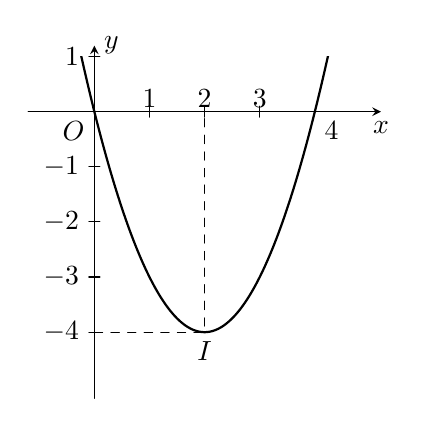
\begin{tikzpicture}[scale=0.7, line join=round, line cap=round, >=stealth]
				\tikzset{every node/.style={scale=1}}
				\def\xmin{-1}\def\xmax{5}\def\ymin{-5}\def\ymax{1}
				\draw[->] (\xmin-0.2,0)--(\xmax+0.2,0) node[below]{$x$};
				\draw[->] (0,\ymin-0.2)--(0,\ymax+0.2) node[right]{$y$};
				\draw (0,0) node[below left]{$O$};
				\foreach \x in {1,2,3}\draw (\x,0.1)--(\x,-0.1) node[above]{$\x$};
				\draw (4,0) node[below right]{$4$};
				\foreach \y in {-4,-3,-2,-1,1}\draw (0.1,\y)--(-0.1,\y) node[left]{$\y$};
				\clip (\xmin,\ymin) rectangle (\xmax,\ymax);
				\draw[thick,smooth,samples=200,domain=\xmin:\xmax] plot (\x,{1*((\x)^2)+-4*\x+0});
				\draw[dashed] (0,-4)--(2,-4)--(2,0);
				\draw (2,-4) node[below]{$I$};
			\end{tikzpicture}
	\end{center}}
	\loigiai{
		\begin{itemize}
			\item  Tập xác định $\mathscr{D}= \mathbb{R}$.
			\item  Đỉnh $I(-1; -4)$.
			\item  Trục đối xứng là đường thẳng $x=-1$.
			\item  Giao điểm với trục $Oy$ là $A(0;-3)$, giao điểm với trục $Ox$ là $B(1 ; 0), C(-3 ; 0)$.
			Ta có đồ thị như hình sau
			\begin{center}
				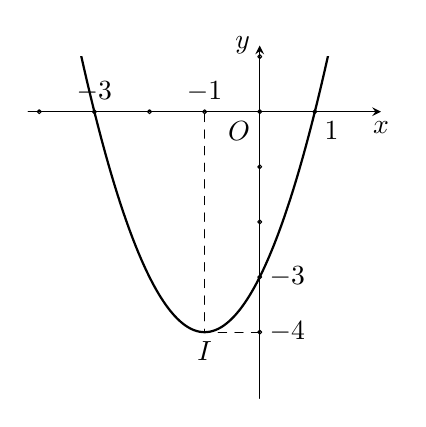
\begin{tikzpicture}[scale=0.7, line join=round, line cap=round, >=stealth]
					\tikzset{every node/.style={scale=1}}
					\def\xmin{-4}\def\xmax{2}\def\ymin{-5}\def\ymax{1}
					\draw[->] (\xmin-0.2,0)--(\xmax+0.2,0) node[below]{$x$};
					\draw[->] (0,\ymin-0.2)--(0,\ymax+0.2) node[left]{$y$};
					\draw (0,0) node[below left]{$O$};
					\foreach \x in {-3,-1}\draw (\x,0) node[above]{$\x$};
					\foreach \x in {-4,-3,-2,-1,1}\draw (\x,0) circle (1pt);
					\draw (1,0) node[below right]{$1$};
					\foreach \y in {-4,-3}\draw (0,\y) node[right]{$\y$};
					\foreach \y in {-4,-3,-2,-1,0,1}\draw (0,\y)circle (1pt);
					\clip (\xmin,\ymin) rectangle (\xmax,\ymax);
					\draw[thick,smooth,samples=200,domain=\xmin:\xmax] plot (\x,{1*((\x)^2)+2*\x-3});
					\draw[dashed] (0,-4)--(-1,-4)--(-1,0);
					\draw (-1,-4) node[below]{$I$};
				\end{tikzpicture}
			\end{center}
			
		\end{itemize}
	}
\end{ex}
%-------------------------------------------------
\begin{ex}%[0D7H3-1]%[Dự án đề kiểm tra Toán Khối 10 GHK2 NH23-24-Dot1-Lê Quốc Dũng]%[DeSo6-KNTT]
	%Câu 2. 
	Cho phương trình $\left(\sqrt{x^2+2x-3}-2 x+2\right)^2+(2-\sqrt{x+3})^2=0$. (*).\\
	Khi đó 
	\choiceTF
	{Điều kiện: $x \geq-3$}
	{Phương trình (*) có $3$ nghiệm phân biệt}
	{$x=\dfrac{7}{3}$ là nghiệm của phương trình $(*)$}
	{\True Nghiệm của phương trình $\left(*\right)$ nhỏ hơn $2$}
	\loigiai{
		Điều kiện $\heva{&x^2+2x-3\geq 0\\&x+3\geq 0}\Leftrightarrow \heva{&\hoac{&x\leq -3\\&x\geq 1}\\&x\geq -3}
		\Leftrightarrow \hoac{&x=3\\&x\geq 1}$.\\
		Ta có $\left(\sqrt{x^2+2 x-3}-2 x+2\right)^2+(2-\sqrt{x+3})^2=0 \Leftrightarrow \heva{&\sqrt{x^2+2x-3}-2 x+2=0 \\ &2-\sqrt{x+3}=0.}$\\
		Phương trình $2-\sqrt{x+3}=0 \Leftrightarrow \sqrt{x+3}=2$ có nghiệm $x=1$.\\
		Ta có $\sqrt{x^2+2x-3}-2 x+2=0 \Leftrightarrow \sqrt{x^2+2x-3}=2 x-2$\quad (2)\\
		Bình phương hai vế phương trình (2) ta có:\\
		$x^2+2x-3=4x^2-8x+4 \Leftrightarrow 3x^2-10x+7=0 \Leftrightarrow x=1$ hoặc $x=\dfrac{7}{3}$ (đều thoả mãn $2x-2 \geq 0$).\\
		Tuy nhiên chỉ có $x=1$ thoả mãn phương trình $2-\sqrt{x+3}=0$.\\
		Vậy tập nghiệm của phương trình ban đầu là $S=\{1\}$.
	}
\end{ex}
%-------------------------------------------------
\begin{ex}%[0H9H3-3]%[Dự án đề kiểm tra Toán Khối 10 GHK2 NH23-24-Dot1-Lê Quốc Dũng]%[DeSo6-KNTT]
	%Câu 3. 
	Cho tam giác $MNP$ có phương trình đường thẳng chứa cạnh $MN$ là $2x+y+1=0$, phương trình đường cao $MK$ $(K \in NP)$ là $x+y-1=0$, phương trình đường cao $NQ$ $(Q \in MP)$ là $3x-y+4=0$. Khi đó
	\choiceTF
	{\True Điểm $M$ có toạ độ là $(-2; 3)$}
	{\True Điểm $N$ có toạ độ là $(-1; 1)$}
	{Phương trình đường thẳng $NP$ là $2x-y+3=0$}
	{Phương trình đường thẳng $MP$ là  $2x+3 y-5=0$}
	\loigiai{
		\begin{itemize}
			\item  Toạ độ của điểm $M$ là nghiệm của hệ phương trình $\heva{&2x+y+1=0 \\ &x+y-1=0} \Leftrightarrow\heva{&x=-2 \\ &y=3.}$\\
			Suy ra điểm $M$ có toạ độ là $(-2 ; 3)$. 
			\item  Toạ độ của điểm $N$ là nghiệm của hệ phương trình $\heva{&2x+y+1=0 \\ &3 x-y+4=0} \Leftrightarrow\heva{&x=-1 \\ &y=1.}$ \\
			Suy ra điểm $N$ có toạ độ là $(-1 ; 1)$.
			\item  Đường cao $MK$ có véc-tơ pháp tuyến là $\overrightarrow{n_1}=(1 ; 1)$.\\
			Do đó đường thẳng $NP$ nhận $\overrightarrow{n_2}=(1;-1)$ là véc-tơ pháp tuyến.\\
			Phương trình đường thẳng chứa cạnh $NP$ đi qua điểm $N(-1 ; 1)$ và có véc-tơ pháp tuyến $\overrightarrow{n_2}=(1;-1)$ là $(x+1)-(y-1)=0 \Leftrightarrow x-y+2=0$.
			\item  Đường cao $NQ$ có véc-tơ pháp tuyến là $\overrightarrow{n_3}=(3 ;-1)$.\\
			Do đó đường thẳng $MP$ nhận $\overrightarrow{n_4}=(1; 3)$ là véc-tơ pháp tuyến.\\
			Phương trình đường thẳng chứa cạnh $MP$ đi qua điểm $M(-2; 3)$ và có véc-tơ pháp tuyến $\overrightarrow{n_4}=(1 ; 3)$ là $(x+2)+3(y-3)=0 \Leftrightarrow x+3y-7=0$.
		\end{itemize}
	}
\end{ex}
%-------------------------------------------------
\begin{ex}%[0H9H4-3]%[Dự án đề kiểm tra Toán Khối 10 GHK2 NH23-24-Dot1-Lê Quốc Dũng]%[DeSo6-KNTT]
	%Câu 4. 
	Cho đường tròn $(C)$ có tâm $I(-1; 2)$ và tiếp xúc với đường thẳng $\Delta: x-2y+7=0$. Khi đó
	\choiceTF
	{$d(I, \Delta)=\dfrac{3}{\sqrt{5}}$}
	{\True Đường kính của đường tròn có độ dài bằng $\dfrac{4}{\sqrt{5}}$}
	{\True Phương trình đường tròn là $(x+1)^2+(y-2)^2=\dfrac{4}{5}$}
	{Đường tròn $(C)$ tiếp xúc với đường thẳng $\Delta$ tại điểm có hoành độ lớn hơn $0$}
	\loigiai{
		\begin{itemize}
			\item  $(C)$ có tâm $I$ và tiếp xúc $\Delta$ nên có bán kính $R=d(I, \Delta)=\dfrac{|-1-4+7|}{\sqrt{1+4}}=\dfrac{2}{\sqrt{5}}$.\\
			Suy ra đường kính bằng  $2R=\dfrac{4}{\sqrt{5}}$.
			\item  Phương trình đường tròn $(C)$ là  $(x+1)^2+(y-2)^2=\dfrac{4}{5}$. \\
			\item  Đường tròn $(C)$ tiếp xúc với đường thẳng $\Delta$ tại điểm có hoành độ nhỏ hơn $0$.\\
			Gọi $A(x_A;y_A)$ là điểm tiếp xúc giữa $(C)$ và $\Delta$.\\
			Ta có:
			\begin{itemize}
				\item $\overrightarrow{IA}=(x_A+1;y_A-2)$;
				\item $\Delta$ có véc-tơ pháp tuyến là $\vec{n}=(1;-2)$ nên có véc-tơ chỉ phương là $\vec{a}=(2;1)$.
			\end{itemize}
			Vì $\overrightarrow{IA} \perp \vec{a}$ và $A\in \Delta$ nên ta có hệ phương trình $\heva{&2x_A+y_A=0\\&x_A-2y_A=-7}\Leftrightarrow\heva{&x_A=-\dfrac{7}{5}\\&y_A=\dfrac{14}{5}}$.	
		\end{itemize}
	}
\end{ex}
%-------------------------------------------------


\Closesolutionfile{ans}
\Closesolutionfile{ansbook}

\begin{center}
	\textbf{\textsf{BẢNG ĐÁP ÁN ĐÚNG SAI}}
\end{center}
\input{Ansbook/DapanDS}

\subsection{Phần tự luận}

\hienthiloigiaibt
%%%=============BT_1=============%%%
\begin{bt}%[0D3H1-7]%[Dự án đề kiểm tra Toán khối 11 GHKII NH23-24-Dot 1- Quan Ón]%[Deso6 - KNTT]
	Một cửa hàng bán kính với giá mỗi cái là $50\,\,000$ đồng. Với giá bán này thì mỗi ngày cửa hàng chỉ bán được $40$ cái. Cửa hàng dự định giảm giá bán, ước tính nếu cửa hàng cứ giảm mỗi cái $1\,\,000$ đồng thì số bánh bán tăng thêm được là $10$ cái. Biết rằng giá nhập về ban đầu cho mỗi cái là $30\,\,000$ đồng. Giá bán để cửa hàng thu được lợi nhuận cao nhất bằng bao nhiêu?
	\loigiai{
		Gọi $x$ (đồng) là giá bán thực tế của mỗi cái bánh. $(30\,\,000 \leq x \leq 50\,\,000)$.\\
		Tương ứng với giá bán $x$ thì số bánh bán được là 
		$$ 40 + \dfrac{10}{1000}(50000 - x) = -\dfrac{1}{100}x + 540. $$
		Gọi $f(x)$ là hàm lợi nhuận thu được ($f(x)$: đồng), ta có
		$$ f(x) = \left(-\dfrac{1}{100}x + 540\right)\cdot (x - 30000) = -\dfrac{1}{100}x^2 + 840x - 16200000. $$
		Giá trị lớn nhất của hàm  $f(x)$ là $144\,\,0000$ có được khi $x = 42\,\,000$ đồng.\\
		Vậy với giá bán $42\,\,000$ đồng một cái bánh thì cửa hàng thu được lợi nhuận lớn nhất.
	}
\end{bt}

%%%=============BT_2=============%%%
\begin{bt}%[0D3H2-6]%[Dự án đề kiểm tra Toán khối 11 GHKII NH23-24-Dot 1- Quan Ón]%[Deso6 - KNTT]
	Tổng chi phí $P$ (đơn vị: nghìn đồng) để sản xuất $x$ sản phẩm được cho bởi biểu thức $P = x^2 + 30x + 3300$; giá bán một sản phẩm là $170$ nghìn đồng. Số sản phẩm được sản xuất trong khoảng nào để đảm bảo nhà sản xuất không bị lỗ (giả sử các sản phẩm được bán hết)?
	\loigiai{
		Khi bán hết $x$ sản phẩm thì số tiến thu được là $170x$ (nghìn đồng).\\
		Điều kiện để nhà sản xuất không bị lỗ là
		$$ 170x \geq x^2 + 30x + 3300 \Leftrightarrow x^2 - 140x + 3300 \leq 0. $$
		Xét $x^2  -140x + 3300 = 0 \Rightarrow \hoac{&x = 30\\&x = 110.}$\\
		Bảng xét dấu
		\begin{center}
			
\begin{tikzpicture}[scale=1, font=\footnotesize, line join=round, line cap=round, >=stealth]
				\tkzTabInit[nocadre=false,lgt=3.2,espcl=2,deltacl=0.6]
				{$x$ /0.6,$x^2 - 140x + 3300$ /0.6}
				{$-\infty$,$30$,$110$,$+\infty$}
				\tkzTabLine{,+,0,-,0,+}
			\end{tikzpicture}
		\end{center}
		Ta có $x^2 - 140x + 3300 \leq 0 \Leftrightarrow x \in [30;110]$.\\
		Vậy nếu nhà sản xuất làm ra từ $30$ đến $110$ sản phẩm thì họ sẽ không bị lỗ.
	}
\end{bt}

%%%=============BT_3=============%%%
\begin{bt}%[0D7H3-2]%[Dự án đề kiểm tra Toán khối 11 GHKII NH23-24-Dot 1- Quan Ón]%[Deso6 - KNTT]
	Tìm nghiệm phương trình sau $\sqrt{x + 2\sqrt{x-1}} = x+\dfrac{1}{4}$.
	\loigiai{
		Ta có
		\begin{eqnarray*}
			\sqrt{x + 2\sqrt{x-1}} = x+\dfrac{1}{4} 
			&\Rightarrow& \sqrt{x - 1 + 2\sqrt{x-1} + 1} = x + \dfrac{1}{4}\\
			&\Rightarrow& \sqrt{\left(\sqrt{x-1} - 1\right)^2} = x + \dfrac{1}{4}\\
			&\Rightarrow& \sqrt{x-1} - 1 = x + \dfrac{1}{4}\\
			&\Rightarrow& \sqrt{x-1} = x + \dfrac{3}{4}\\
			&\Rightarrow& \heva{&x - \dfrac{3}{4} \geq 0\\&x - 1 = x^2 - \dfrac{3}{2}x + \dfrac{9}{16}}\\
			&\Rightarrow& \heva{&x \geq \dfrac{3}{4}\\&x^2 - \dfrac{5}{2}x + \dfrac{25}{16}}\\
			&\Rightarrow& \heva{&x \geq \dfrac{3}{4}\\&x = \dfrac{5}{4} \textrm{ (loại).}}
		\end{eqnarray*}
		Vậy phương trình đã cho vô nghiệm.
	}
\end{bt}

%%%=============BT_4=============%%%
\begin{bt}%[0H5H2-3]%[Dự án đề kiểm tra Toán khối 11 GHKII NH23-24-Dot 1- Quan Ón]%[Deso6 - KNTT]
	Cho ba điểm $A(-1;1)$, $B(2;1)$, $C(-1;-3)$.\\
	Xác định điểm $D$ sao cho tứ giác $ABCD$ là hình bình hành.
	\loigiai{
		Gọi $D(x;y) \Rightarrow \overrightarrow{DC} = (-1-x;-3-y)$, $\overrightarrow{AB} = (3;0)$.\\
		Vì $ABCD$ là hình bình hành nên
		$$ \overrightarrow{AB} = \overrightarrow{DC} \Leftrightarrow \heva{&-1-x = 3\\&-3-y = 0} \Leftrightarrow \heva{&x = -4\\&y = -3} \Rightarrow D(-4;-3).$$
	}
\end{bt}

%%%=============BT_5=============%%%
\begin{bt}%[0H9V3-7]%[Dự án đề kiểm tra Toán khối 11 GHKII NH23-24-Dot 1- Quan Ón]%[Deso6 - KNTT]
	Trong mặt phẳng với hệ trục tọa độ $Oxy$, cho tam giác $ABC$ cân tại $A$ với $BC = 4\sqrt{2}$. Các đường thẳng $AB$ và $AC$ lần lượt đi qua các điểm $M\left(1;-\dfrac{5}{3}\right)$ và $N\left(0;\dfrac{18}{7}\right)$. Biết đường cao $AH$ có phương trình $x + y - 2 = 0$ và điểm $B$ có hoành độ dương. Đường thẳng $BC$ có phương trình là gì?
	\loigiai{
		\immini{
			Gọi $N'$ đối xứng với $N\left(0;\dfrac{18}{7}\right)$ qua $AH$, suy ra $N' \in AB$.\\
			$NN'$ đi qua $N\left(0;\dfrac{18}{7}\right)$ và vuông góc với $AH$ nên có phương trình $x - y + \dfrac{18}{7} = 0$.\\
			Khi đó tọa độ giao điểm $I$ của $NN'$ và $AH$ là nghiệm của hệ
			$$ \heva{&x - y + \dfrac{18}{7} = 0\\&x + y - 2 = 0} \Leftrightarrow \heva{&x = - \dfrac{2}{7}\\&y = \dfrac{16}{7}} \Rightarrow I\left(-\dfrac{2}{7};\dfrac{16}{7}\right).$$
		}{
			\begin{tikzpicture}[>=stealth,line join=round,line cap=round,font=\footnotesize,scale=1]
				\path 
				(2,3.4) coordinate (A)
				(0,0) coordinate (B)
				(4,0) coordinate (C)
				($(B)!(A)!(C)$) coordinate (H)
				($(A)!0.3!(B)$) coordinate (N')
				($(A)!0.3!(C)$) coordinate (N)
				($(A)!0.7!(B)$) coordinate (M)
				(intersection of N--N' and A--H) coordinate (I)
				;
				\draw (A)--(B)--(C)--(A)--(H) (N')--(N);
				\foreach \l/\g in {A/90,B/-135,C/-45,H/-90,M/180,N'/180,N/0,I/-45}
				\draw[fill=black] (\l) circle (1pt) +(\g:.3) node{$\l$};
				\pic[draw,angle radius=2mm,angle eccentricity=1.5] {right angle = A--H--B};
			\end{tikzpicture}
		}
		\noindent
		Do $I$ là trung điểm của $NN'$ suy ra $N'\left(-\dfrac{4}{7};2\right)$.\\
		Khi đó $AB$ đi qua $M\left(1;-\dfrac{5}{3}\right)$ và $N'\left(-\dfrac{4}{7};2\right)$ nên có phương trình $7x + 3y - 2 = 0$.\\
		Gọi $B(-1+3t; 3-7t) \in AB$ với $t > \dfrac{1}{3}$.\\
		Khi đó, ta có
		$$ \mathrm{d}(B,AH) = \dfrac{BC}{2} = 2\sqrt{2} \Leftrightarrow \dfrac{\left| -1 + 3t + 3 - 7t - 2 \right|}{\sqrt{2}} = 2\sqrt{2} \Leftrightarrow \hoac{&t = 1\\&t = -1.} $$
		Do $t > \dfrac{1}{3}$ nên $t = 1$ suy ra $B(2;-4)$.\\
		Đường thẳng $BC$ đi qua $B(2;-4)$ và vuông góc với $AH$ nên có phương trình $x - y - 6 = 0$.
	}
\end{bt}

%%%=============BT_6=============%%%
\begin{bt}%[0H9H4-3]%[Dự án đề kiểm tra Toán khối 11 GHKII NH23-24-Dot 1- Quan Ón]%[Deso6 - KNTT]
	Trong hệ tọa độ $Oxy$, cho đường tròn $(C)$ có phương trình $x^2 + y^2 -8x + 4y - 5 = 0$, viết phương trình tiếp tuyến với $(C)$ biết tiếp tuyến có hệ số góc âm và tiếp tuyến tạo với các trục tọa độ một tam giác cân.
	\loigiai{
		Đường tròn $(C)$ có tâm $I(4;-2)$, bán kính $R = 5$.\\
		Đường thẳng $d$ tạo với các trục tọa độ một tam giác cân thì hệ số góc của $d$ là $\hoac{&k = 1 \textrm{ (loại)}\\&k = -1 \textrm{ (thỏa mãn).}}$\\
		Khi $k = -1$ thì $d$ có dạng $y = -x + m \Leftrightarrow x + y - m = 0$.\\
		Vì $d$ là tiếp tuyến của $(C)$ nên
		$$ \mathrm{d}(I,d) = R \Leftrightarrow \dfrac{\left| 4 - 2 - m \right|}{\sqrt{2}} = 5 \Leftrightarrow \left| m - 2\right| = 5\sqrt{2} \Leftrightarrow \hoac{&m = 5\sqrt{2} + 2\\&m = -5\sqrt{2} + 2.}$$
		Suy ra $d$ có phương trình $x + y - 5\sqrt{2} - 2 = 0$; $x + y + 5\sqrt{2} - 2 = 0$.
	}
\end{bt}









